\section{Operators}\label{sec:operators}
As described in section~\ref{sec:genetics}, genetic operators are used to create
new individuals.
This section presents crossover and mutation genetic operators
that are used for the individual representation from section~\ref{sec:coding}.

\subsection{Crossover}\label{subsec:crossover}

Novel crossover approach proposed in this thesis
creates a new individual by weighted vector addition of the parent's stochastic vectors followed by a normalization back to the stochastic vector.
Using notation from section~\ref{sec:coding}, that is
$PS_{rk}$ for painting sequence random key vector,
$SO_{rk}$ for slicing order random key vector and
$OR_{prob}$ for orientation probabilities matrix,
we can define crossover for two parents $A$, $B$ and offspring $C$ as

\begin{equation}
    \|w_A A_{PS_{rk}} + w_B B_{PS_{rk}}\| = C_{PS_{rk}}\,,
    \label{eq:crossover-psrk}
\end{equation}

\begin{equation}
    \|w_A A_{SO_{rk}} + w_B B_{SO_{rk}}\| = C_{SO_{rk}}\,,
    \label{eq:crossover-sork}
\end{equation}

\begin{equation}
    \|P^T(w_A A_{OR_{prob}i:} + w_B B_{OR_{prob}i:})\| = C_{OR_{prob}i:}\,,
    \label{eq:crossover-orprob}
\end{equation}

where $\|\cdot\|$ is normalization to the stochastic vector, $+$ is vector addition, $w_A, w_B \in \real$ are weights,
$P \in \real^{N-1}$ is orientation penalization vector with $N$ being instance size, notation $X_{i:}$ means $i$-th row of a matrix $X$
and multiplying a vector by a scalar multiplies each element of the vector by that scalar.

Example of crossover for painting sequence random key and slicing order random key, eq.~\ref{eq:crossover-psrk} and~\ref{eq:crossover-sork},
is in figure~\ref{fig:crossover-random-keys}.
An example of crossover for orientation probabilities, eq.~\ref{eq:crossover-orprob}, is in figure~\ref{fig:crossover-orientation-probabilities}.

The crossover implementation described above has multiple parts – vector sum, weights, orientation penalization and normalization.
Following are arguments for incorporating each of those parts into a crossover.

\subsubsection*{Vector addition and normalization}

Adding and then normalizing vectors to stochastic vectors differs from other crossover implementations.
For example, in one-point-crossover~\cite{hollandAdaptationNaturalArtificial1975} and
uniform crossover~\cite{uniformCrossover1989}, parts of the parent chromosomes are copied directly without any modification to form an offspring.

By using a stochastic vector for painting sequence random keys, slicing order random keys and rows of an orientation probability matrix,
we can interpret each of them as a probability mass function.
Next, by implementing the crossover as vector addition followed by normalization, we can
say the crossover approximates a probability mass function of some distribution from two samples, i.e.,two parents.
Over the course of the multiple generations, more and more samples are added to this approximation.
Thus, each part of the chromosome tries to approximate probability mass function
that produces (sub)-optimal painting placement solution.

Going back to the schema theorem described subsection~\ref{subsec:schema-theorem},
we can say that the crossover proposed in this thesis does not prefer schemata with any particular order
and that length of a schema does not matter.

Preference for schemata with short length in one-point-crossover~\cite{hollandAdaptationNaturalArtificial1975}
stems from the fact that a chromosome is split at the particular position.
This idea of splitting a chromosome is not present in the proposed approach.
For example, let us consider slicing order random key vector $A_{rk} = 0, 0.2, 0.7, 0.1$.
Using the decoding procedure described in~\ref{subsec:individual-decoding},
$A_{rk}$ decodes to $A = 1, 4, 2, 3$.
Then, $A$ belongs to the schema $S_1 = 1, \_, \_, \_$ and also to schema $S_2 = 1, \_, \_, 3$.
$S_1$ has order 1 and $S_2$ has order 4.
Let us apply crossover to $A_{rk}$ and $B_{rk} = b_1, b_2, b_3, b_4$.
Result is $\|b_1, 0.2+b_2, 0.7+b_3, 0.1+b_4\|$.
We cannot make any assumptions whether the result belongs to $S_1$ or $S_2$, as it purely depends on on $B_{rk}$.
Additionally, we cannot predict probability whether $S_1$ or $S_2$ survives, i.e., they will be still present in the crossover result.
However, using one-point-crossover, it would depend on the position of the split.

Lastly, the proposed crossover does not prefer any particular order of schemata.
This is the same as in one-point-crossover, which has only preference for shorter schemata.


\subsubsection*{Weights}
Adding weights $w_A$ and $w_B$ determine the preference for transfer of information from one parent then the other.
The weights are calculated using a cost function $c$ from eq.~\ref{eq:objective} as

\begin{equation}
    w_A = \dfrac{c(B)}{c(A)+{c(B)}}, w_B = 1 - w_A\,.
    \label{eq:weights}
\end{equation}

Thus, parent with better performance in the population, i.e., having lower cost function,
has more influence on what genes are being transferred to the offspring.

Adding $w_A$ and $w_B$ prevents from creating offsprings that do not share the advantageous schemata.
For example, considering only one stochastic vector of length 3 as chromosome,
it might be advantageous having high value for the first value in the chromosome, e.g., $A=\langle 0.7, 0.1, 0.2 \rangle$.
On the other hand, poorly performing individual might be $B=\langle 0.1, 0.3, 0.6 \rangle$.
Without weights, $\| A+B\| = \langle 0.4, 0.2 , 0.4 \rangle$.
Adding weights according to the eq.~\ref{eq:weights} penalize the transfer of schemata that perform poorly.

\subsubsection*{Orientation penalization}

Another part of the crossover used in orientation probabilities matrix is the penalization vector $P$.
As mentioned in section~\ref{sec:layout-construction}, each individual is decoded to a slicing tree
whose internal nodes contain type of the cut – $H$ for horizontal, $V$ for vertical
and $*$ for wildcard, that can take up any value $H$ or $V$.
Vector $P$ controls the preference for each type of the cut.
For example, setting $P= \langle 1,1,0.5 \rangle$ penalize only the wildcard $*$.
On the other hand, setting $P= \langle 1,1,1 \rangle$ removes any penalization.

The main reason for introducing $P$ is to limit the spread of wildcard $*$ in population,
making its appearance only at the most advantageous parts of the genes.

\begin{figure}[!htp]
    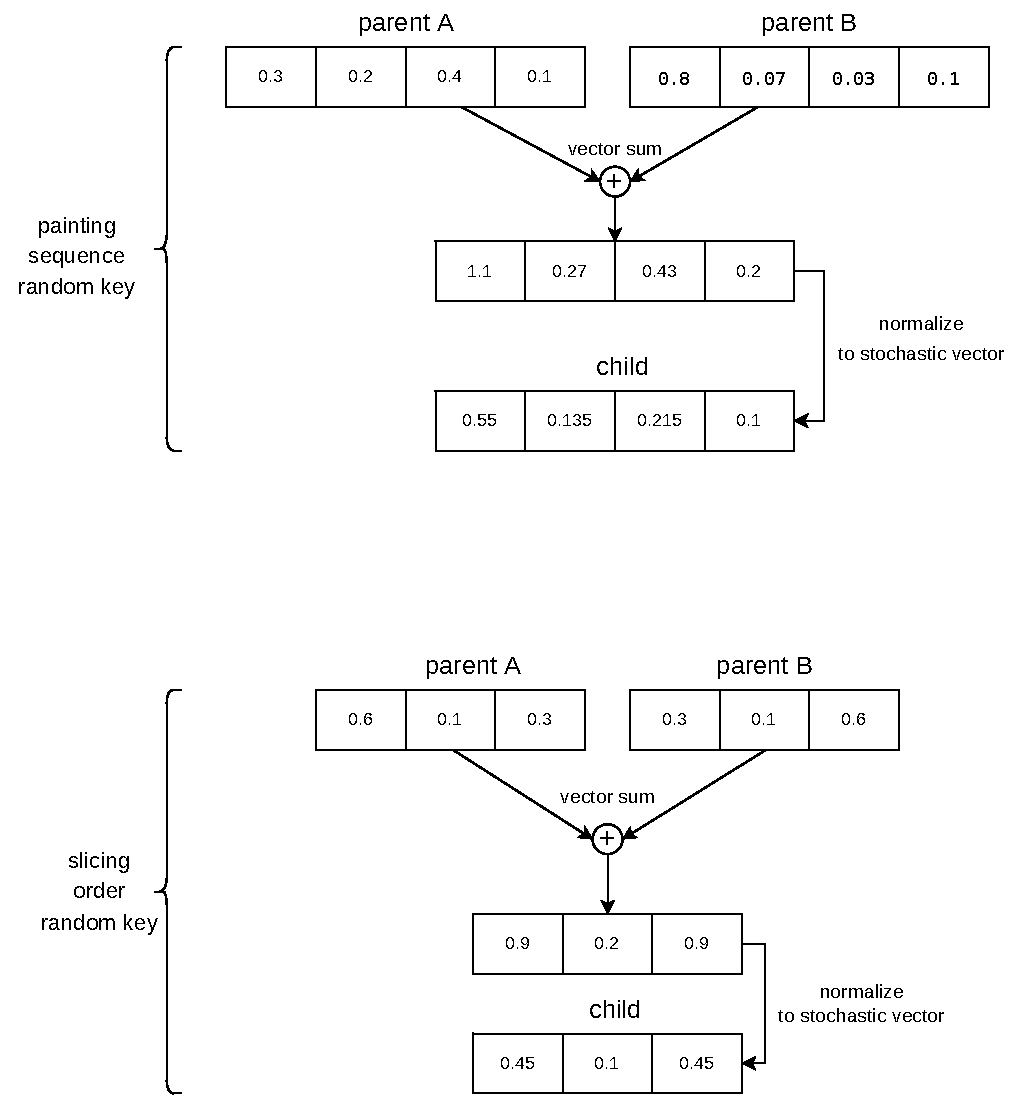
\includegraphics[width=1.0\textwidth, left]{crossover_random_keys}\caption{
        Crossover example for painting sequence and slicing order random keys.
        The procedure is the same for both – sum weighted parent vectors and then normalize to stochastic vector.
    }
    \label{fig:crossover-random-keys}
\end{figure}

\begin{figure}[!htp]
    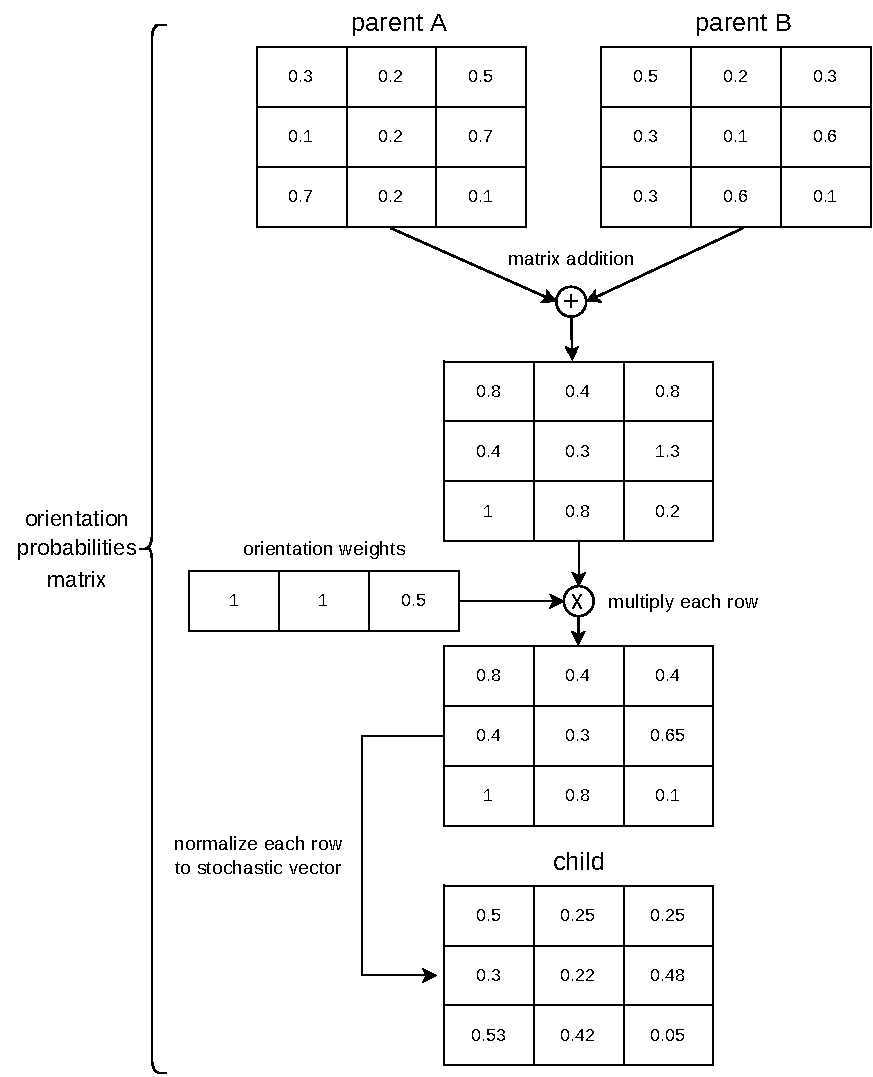
\includegraphics[width=0.85\textwidth, left]{crossover_orientation_probabilities}\caption{
        Crossover example for orientation probabilities. The procedure is first to sum weighted parent matrices,
        then multiply the matrix with orientation penalization vector and normalize each row to a stochastic vector.}
    \label{fig:crossover-orientation-probabilities}
\end{figure}

\subsection{Mutation}\label{subsec:mutation}

Mutation can happen on all three genes of a chromosome – painting sequence random key $PS_{rk}$,
slicing order random key $SO_{rk}$ and orientation probabilities $OR_{prob}$.
Due to the coding described in section~\ref{sec:coding}, $PS_{rk}$, $SO_{rk}$ and rows of $OR_{prob}$ are stochastic vectors.
We use this common trait and define the mutation operator for a stochastic vector as follows.

\begin{enumerate}
    \item Replace one randomly chosen element with a uniformly generated value from $\langle 0,1 \rangle$.
    \item Normalize to stochastic vector.
\end{enumerate}

With the definition of the mutation operator for a stochastic vector above, the mutation operator for an individual is defined as follows.

\begin{enumerate}
    \item Choose one of $PS_{rk}$, $SO_{rk}$, $OR_{prob}$ at random.
    \item If $PS_{rk}$ or $SO_{rk}$ is chosen, apply mutation operator for a stochastic vector.\\
    If $OR_{prob}$ is chosen, select one row at random and apply a mutation operator for a stochastic vector.
\end{enumerate}

It is important to mention how to interpret a mutation operator.
As mentioned in section~\ref{sec:layout-construction}, an individual is decoded to a slicing tree.
Mutation modifies this tree.
First, if applied to $OR_{prob}$, the value of an inner node of the tree might change.
That means a change in a type of cut – $H$, $V$, or $*$.
Second, if applied to $PS_{rk}$, the value of leaves in the tree might change.
Lastly, if applied to $SO_{rk}$, the whole structure of a tree might change.

As described above, even changing one value can result in a completely different layout after decoding.
This is the reason for defining mutation as such – to damage the chromosome as little as possible.
An example of a mutation that happens on all tree parts at once is in figure~\ref{fig:mutation}.


\begin{figure}[!htp]
    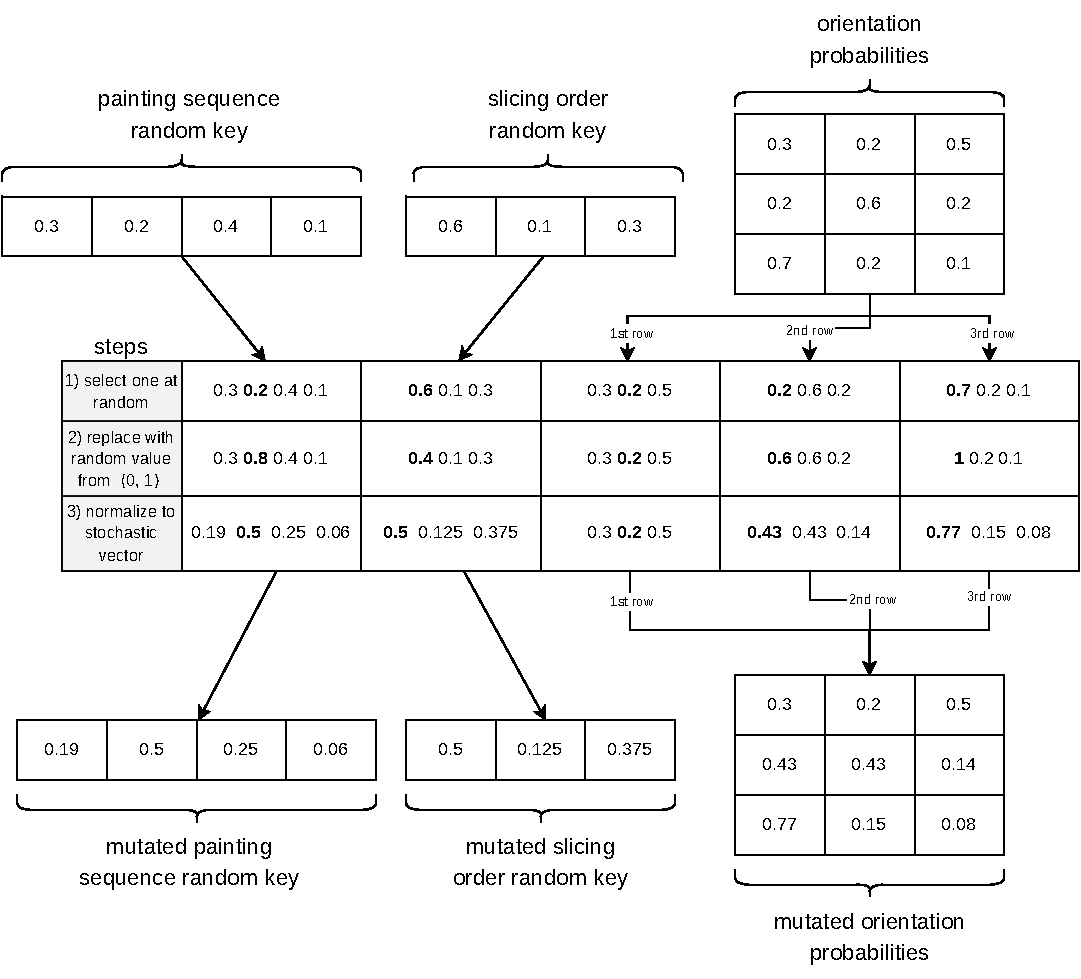
\includegraphics[width=1.0\textwidth, left]{muation}\caption{
        Example of a mutation on all three parts of a chromosome.
        Since all parts can be treated as a stochastic vector, the same procedure
        is used for all of them – replace one value randomly and then normalize to a stochastic vector.
    }
    \label{fig:mutation}
\end{figure}

